\section{Working principles of disk brake systems}

		This section will give a short explanation of how disk breaks works as the vast majority of cars and motorcycles nowadays are equiped with this technology instead of the outdated drum scheme.
		\par
		In general terms we can make an analogy of how disk brake works with how bicycles brakes works. In a bicycle the brake calipers squeeze the wheels in order to promove deceleration to the wheel and reduce the bike speed. In disk breaks the calipers apply pressure to the rotor \textit{disk}, the rotor is directly connected to the wheel spinning at the same speed, this way the system decelerates the rotor and the wheel trying to reduce the vehicle speed. In car disk breaks there is a component called pad, as seen on Figure \ref{fig:working-of-disk-breaks} pads are located between the calipers and the rotor. Pads have the functionality to reduce the wear generated by friction in the rotor. In normal conditions during proper maintenance calipers are hardly-ever replaced, pads are replaced every once in a while and disks are replaced also every once in a while but less frequently than pads.

		\begin{figure}[htbp]
			\centering
				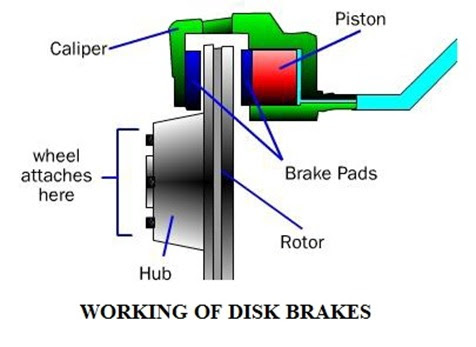
\includegraphics[scale=0.55]{figuras/fig-disk_brake_working}
			\caption{Schematic for disk brake systems \cite{fig-working-of-disk-breaks}}
			\label{fig:working-of-disk-breaks}
		\end{figure}
